\chapter{Evaluation}\label{sec:evaluation}

\epigraph{``All models are wrong but some are useful``}{\textit{– George Box}}

In this chapter, we present the results obtained from our approach. Additionally, we compare the developed approach with state-of-the-art strategies: evolutionary algorithms and static compound model-based optimization.


% --------------------------------------------------------------------------------------------
% ------------------------------------------------     Experimental setup     
% --------------------------------------------------------------------------------------------
\section{Experimental setup}
    We will begin by introducing a description of the selected optimization problems and applicable approaches for their analysis. Those problems include ZDT, DTLZ and WFG problems suits. 

    % ---------------------------------     Optimization problems
    \subsection{Optimization problems}
    Different optimization approaches need to applied to the numerous types of optimization problems to reduce the comparison bias in the obtained results (direct consequence of the \gls{nfl}). To that mean, we select several comprehensive synthetic benchmark suites for comparison. They are all scalable in the parameter space and some are scalable in the objective space. The problems are designed so that a meaningful comparison can be obtained for optimization techniques. All cases are minimization problems.

    According to \cite{WFGref}, the following properties characterize the optimization problems:
    \begin{itemize}
        \item \emph{Modality} is a property of the objective surface. Test problems are either unimodal, with one global optimum, or multimodal, with several local optima. Multimodal problems are more complicated than unimodal ones and bear more resemblance with real-world scenarios (Figure \ref{fig:multi_modal_zdt4}). Deceptive objective functions have a special kind of multimodality that has at least two optima — a true optimum and a deceptive optimum — but the majority of the search space favors the deceptive optimum \cite{Deb99}.
        \item A \emph{geometry} of the Pareto optimal front can be convex, linear, concave, mixed, degenerate, disconnected, or some combination of the former. It directly influences the algorithm's performance. 
        \item A \emph{bias} in landscape transformations impacts the search process by biasing the fitness landscape. Bias means that uniformly distributed parameters mapped onto a bias area in objective space. This type of problem can cause challenges if the bias region is far from the Pareto optimal front (Figure \ref{fig:bias_area_wfg1}).
        \item \emph{Many-to-one} fitness mapping means that different parameter vectors can produce the same objective vector. This property makes the search more difficult to optimize because it leads to situation when most solutions produce the same result.
        \item \emph{Not separability } of the problem means that it can not be solved if consider it as a separate optimization problems for each objective.
    \end{itemize}

    \begin{figure}
        \centering
        \begin{subfigure}{\textwidth}
            \begin{subfigure}{0.64\textwidth}
                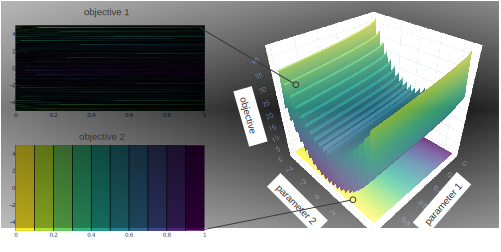
\includegraphics[width=\textwidth]{content/images/utility/multi_modal_zdt4}
                \caption{}
                \label{fig:multi_modal_zdt4}
            \end{subfigure} 
            \begin{subfigure}{0.35\textwidth}
                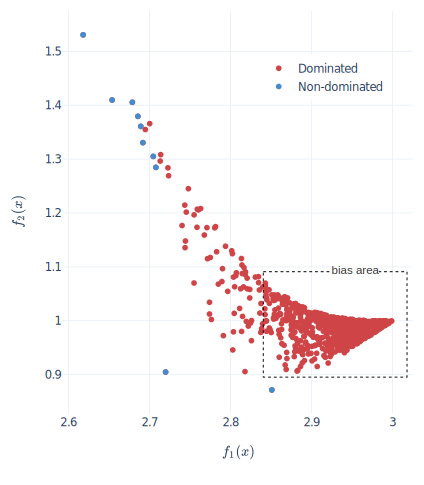
\includegraphics[width=\textwidth]{content/images/utility/bias_area_wfg1}
                \caption{}
                \label{fig:bias_area_wfg1}
            \end{subfigure} 
        \end{subfigure} 
        \caption[Example of unimodal, multimodal and bias problems]{\textbf{(a)} Example of ZDT4 problem landscapes with multimodal (\#1) and unimodal objectives (\#2). \textbf{(b)} Example of bias landscape in WFG1 problem. Note how, in this example, the objective vectors are denser far away from Pareto optimal solutions.}
        \label{fig:changing_models}    
    \end{figure}

    % ! [===    Many-to-one, bias, Modality, geometry  ===]
        % -----------------------------  ZDT      
        \paragraph{ZDT}\cite{ZitzlerDT00} is a test suite that consists of a set of two-objective problems and takes its name from its authors Zitzler, Deb and Thiele. In their paper the authors propose a set of 6 different scalable problems all originating from a well thought combination of functions allowing, by construction, to measure the distance of any point to the Pareto front. Each test function involves a particular feature that is known to cause difficulties in the evolutionary optimization process, mainly in converging to the Pareto-optimal front.
        For the evaluation of our combinational surrogate model we selected the following problems:
        \begin{itemize}
            \item ZDT1 has a convex Pareto optimal front.
            \item ZDT2 has a non-convex Pareto optimal front.
            \item ZDT3 adds a discreteness feature to the front. Its Pareto optimal front consists of several noncontiguous convex parts. The introduction of a sine function in this objective function causes discontinuities in the Pareto optimal front, but not in the parameter space.
            \item ZDT4 has 21 local Pareto-optimal fronts and therefore is highly multimodal. It is also called a \textit{multifrontal} problem.
            \item ZDT6 has a non-uniform search space: the Pareto optimal solutions are non-uniformly distributed along the global Pareto front and the density of solutions is lowest near the Pareto optimal front and highest away from the front.
        \end{itemize}


        % -----------------------------   DTLZ
        \paragraph{DTLZ}\cite{DebTLZ05} is an extensive test suite that takes its name from its authors Deb, Thiele, Laumanns, and Zitzler. It was conceived for multi-objective problems with scalable fitness and objective dimensions.  All problems in this test suite are box-constrained, continuous, n-dimensional, multi-objective problems.
        \begin{itemize}
            \item DTLZ1  is one of the most difficult test problems in this test set. DTLZ1 has a flat landscape and the optimal Pareto front lies on a linear hyperplane. 
            \item DTLZ2 is an unimodal problem with a concave Pareto front.
            \item DTLZ3 is a multimodal problem with a concave Pareto front. DTLZ3 is intended to make convergence on the optimal Pareto front more difficult than for DTLZ2.
            \item DTLZ4 is an unimodal problem with a bias toward a dense region of solutions.
            \item DTLZ5 has a bias for solutions close to a Pareto optimal curve. This problem may be easy for an algorithm to solve. Because of its simplicity, it is recommended to use it with a higher number of objectives.
            \item DTLZ6 is a more challenging version of the DTLZ5 problem. It has a non-linear distance function $g()$, which makes it more difficult to find the Pareto optimal front.
            \item DTLZ7 is an unimodal problem for its first objective and multimodal for the rest of its objectives. This problem has a disconnected Pareto optimal front, which decreases the likelihood that an \gls{ea} finds all optimal regions.
        \end{itemize}

        % ------------------------------    WFG
        \paragraph{WFG}\cite{WFGref} is a test suite designed to outperform the previously implemented test suites. Essential improvements have been achieved in a many problems. Also, non-separable, deceptive, and mixed-shape Pareto front problem are included. The WFG test suite was introduced by Simon Huband, Luigi Barone, Lyndon While, and Phil Hingston. 
        WFG includes the following problems:
        \begin{itemize}
            \item WFG1 is an unimodal problem with a convex and mixed Pareto front geometry. 
            \item WFG2 is a non-separable and unimodal problem with a convex and disconnected Pareto front geometry.
            \item WFG3 is a non-separable, unimodal problem for all but its last objective. The last objective is multimodal.
            \item WFG4 is a multimodal problem with a concave Pareto front geometry. The multimodality of this problem has a landscape with large hills that makes optimization more complicated.
            \item WFG5 is a separable problem with a deceptive landscape and a concave Pareto front geometry.
            \item WFG6 is a non-separable and unimodal problem. Its Pareto front geometry is concave. 
            \item WFG7 is a separable, unimodal problem with a concave Pareto front geometry. WFG7 and WFG1 are the only problems that are both separable and unimodal.
            \item WFG8 is a non-separable, unimodal problem with a concave Pareto front geometry.
            \item WFG9 is a multimodal, deceptive, and non-separable problem with a concave Pareto optimal geometry. Similar to WFG6, the non-separability of this problem makes it more complicated than WFG2 and WFG3.
        \end{itemize}


        Base on the properties, we decide that ZDT4, ZDT6, DTLZ4, WFG1, and WFG4 can represent a broader spectre of possible problems (Table \ref{tab:bench_problems}). Also, solutions to these problems provide meaningful insight into how our optimization strategy performs. Therefore, for brevity and more comprehensible discussion, we present full evaluation only of these problems. However, we have condensed results for all mentioned problems in \hyperref[sec:appendix-a]{appendix A}.

        % ==== multi-objective test problems
        \begin{table}[]
            \centering
            \resizebox{\textwidth}{!}{%
                \begin{tabular}{@{}cccccc@{}}
                \toprule
                \multirow{2}{*}{\textbf{Problem}} &
                \multirow{2}{*}{\textbf{Objective}} &
                \multirow{2}{*}{\textbf{Modality}} &
                \multirow{2}{*}{\textbf{Geometry}} &
                \multicolumn{2}{c}{\textbf{Landscape}} \\ \cmidrule(l){5-6}
                            &                 &                      &               & \textbf{Bias}    & \textbf{\begin{tabular}[c]{@{}c@{}}Many-to-one \\ mappings\end{tabular}} \\ \midrule
                \textbf{ZDT4}  & bi-objective    & unimodal, multimodal & convex        & -                & -                                                                        \\
                \textbf{ZDT6}  & bi-objective    & multimodal           & concave       & +                & +                                                                        \\
                \textbf{DTLZ4} & multi-objective & unimodal             & concave       & +                & +                                                                        \\
                \textbf{WFG1}  & multi-objective & unimodal             & convex, mixed & polynomial, flat & +                                                                        \\
                \textbf{WFG4}  & multi-objective & multimodal           & concave       & -                & +                                                                       \\ \bottomrule
                \end{tabular}%
            }
            \caption{Selected multi-objective test problems}
            \label{tab:bench_problems}
        \end{table}


    % ---------------------------------     Optimization search
    \subsection{Optimization search}
    In this thesis, we do not perform explicit parameter tuning for optimization algorithms. While various optimization algorithms could have been used, we selected \glspl{moea} as default optimization techniques for surrogate models. The advantage of \gls{ea}s are that they can be easily modified and can operate on a set of solutions candidates that are well-fitted to approximate the Pareto front. Also, \glspl{ea} can estimate highly complex problems in various use-cases. In this thesis, we used two types of \gls{ea}:

    \begin{enumerate}
        \item The popular evolutionary multi-objective algorithm \emph{NSGA2} \cite{DebAPM00}. We chose this algorithm due to its popularity in \gls{moo}. In all cases, default parameters for the algorithm were used (population size=100, crossover probability=0.95, distribution index for crossover=10.0, mutation probability=0.01, distribution index for mutation=50.0)\cite{francesco_biscani_2019}.
        \item As an alternative MOEA algorithm for optimization, we define \emph{MOEA-Ctrl} that combines MOEA/D \cite{ZhangL07} and NSGA2 algorithms. The characteristic of such an optimization process based on a common solutions population for both algorithms. Our intuition behind this choice is the following: NSGA2 gives stable results with well-distributed points on the Pareto front while MOEA/D has great exploration quality with low generation count. The combination of this algorithm should gain a better trade-off in exploration and exploitation in contrast to individual algorithms' application.  
    \end{enumerate}

    % ---------------------------------    Portfolio
    \subsection{Surrogate portfolio}
    Based on our awareness, we selected the most popular models for a default surrogate portfolio.
    \begin{enumerate}
        \item \textbf{Gaussian Process Regressor}\footnote{{scikit-learn.org}: sklearn.gaussianprocess.GaussianProcessRegressor} it is a multi-objective surrogate model that commonly used in the Bayesian optimization. For this type of model, the initialization should be specified by passing a kernel object, the hyperparameters of which are optimized during extrapolations of the samples.  The kernel for benchmarks is selected from the GPML\cite{RasmussenN10}. Even though this kernel is from another domain, it does give good extrapolation quality for the regression model. Unfortunately, the build time is significant and grows with samples size and dimensionality.
        \item \textbf{Support Vector Regression (SVR)}\footnote{{scikit-learn.org}: sklearn.svm.SVR} single-objective model with Radial-basis function(RBF) kernel. Surrogate based on RBF and SVR are preferred choice for high dimensional problems \cite{akhtar2019efficient}.
        \item \textbf{Multi-layer Perceptron regressor (MLPRegressor)}\footnote{{scikit-learn.org}: sklearn.neural network.MLPRegressor} A neural network is a popular and influential approach to approximate the functions landscape \cite{KOURAKOS201313}.
        \item \textbf{Gradient Boosting Regressor}\footnote{{scikit-learn.org}: sklearn.ensemble.GradientBoostingRegressor} is a single-objective model that uses an ensemble decision tree regressors to produce a single model.
    \end{enumerate}
    
    As a result, for bi-objective problems, there are no more than ten possible surrogate hypotheses (including multi-objective Gaussian Process Regressor). For a benchmark purpose, at each optimization round the surrogate portfolio does not change. 

    % ---------------------------------    Benchmark baseline
    \subsection{Benchmark baseline}
    We compare our approach (TutorM\footnote{{github: Valavanca/ compositional-system-for-hyperparameter-tuning}}) with Hypermapper 2.0\cite{nardi2019practical} that was described in Chapter ref{sec:related}. Hypermapper focuses on multi-objective parameter tuning with various types of parameters. It uses several randomized forest models, one for each objective. The general idea is to scalarize several surrogate models to single-objective criteria and to optimize them as a single-objective problem. In addition, a Bayesian model is used to assist the search for solutions. Hypermapper has successfully been used in autotuning computer vision applications and database optimization. Since the sample size is not specified, we chose to use the default population size for MOEA (100 points).

    In addition to Hypermapper, NSGA2 was chosen as it is one of the most well-known evolutionary algorithms \cite{RamirezRV19}. It is therefore a suitable reference point to which to compare other approaches. As benchmarks, we evaluate two versions of the algorithm that are nearly identical but have a different budget for evaluation:
        \begin{itemize}
            \item Small evaluation budget (1000 functions evaluations) and used as a competing algorithm
            \item Large evaluation budget (10000 and 50000 functions evaluations) and used as a baseline. NSGA2 with 10000 functions evaluations budget used as a baseline for figures with runtime performance, whereas 50000 budget used for final results.
        \end{itemize}


% --------------------------------------------------------------------------------------------
% ---------------------       Benchmark 1: Model-tutor: Portfolio with compositional surrogates 
% --------------------------------------------------------------------------------------------
\section{Benchmark 1: Portfolio with compositional surrogates. Dynamic sampling plan}
    For this first evaluation step, our approach (TutorM) was compared to related approaches (Hypermapper and NSGA2) while solving all three sets of problems described above (ZDT, DTLZ, WFG) for 2 objectives and 2 or 3 parameters. The TutorM includes all features such as dynamic compositional models, surrogate portfolio and validation. 

    The solution quality was evaluated using the following metrics: hypervolume, p-distance, spacing, and number of available non-dominant solutions (ndf size, Chapter \ref{sec:related}). The results we present are the average values obtained after five repetitions. It should also be noted that baseline NSGA2 10k is a static value that is obtained after 10000 function evaluations.

    % -------------------------------------------------------- One case
    \subsection*{One case studies: ZDT6}
    We start by comparing the runtime performance of the approaches. Let us consider runtime optimization for the ZDT6 problem. In Figure \ref{fig:zdt6_dist}, optimization progress and average distance to the Pareto front is shown. 
    
        \begin{figure}[h]
            \centering
            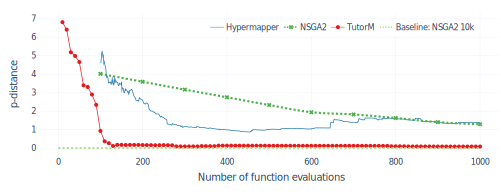
\includegraphics[width=\textwidth]{content/images/zdt6_dist}
            \caption[Results of 5 repetitions for ZDT6: Distance of non-dominant solutions to the real Pareto front]{Results of 5 repetitions for ZDT6: Average distance of non-dominant solutions to the real Pareto front}
            \label{fig:zdt6_dist}
        \end{figure}
        
    It is evident that TutorM considerably outperforms NSGA2 and Hypermapper 2.0 right from the start of the optimization process. Our algorithm quickly reaches optimal and stable results after 300 function evaluations. As can be seen from another approach, Hypermapper began to improve values confidently, but then deteriorated and matched with NSGA2. The presented p-distance is measured from non-dominated solutions (ndf size) that can be found in Figure \ref{fig:zdt6_ndf}. 
    
        \begin{figure}[h]
            \centering
            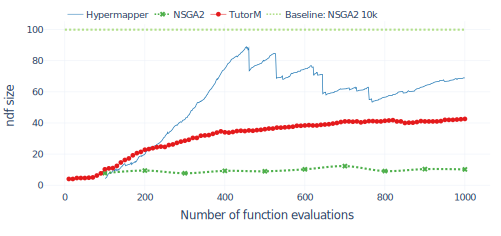
\includegraphics[width=\textwidth]{content/images/zdt6_ndf}
            \caption[Results of 5 repetitions for ZDT6: Size of non-dominant solutions across the entire set of the measured solutions]{Results of 5 repetitions for ZDT6: Size of non-dominant solutions across the entire set of the measured solutions}
            \label{fig:zdt6_ndf}
        \end{figure}
    
    The count of solutions from TutorM grows evenly, reflecting the stability of the search and the ascent to the real Pareto front. On the contrary, Hypermapper has a serrated, unstable track that corresponds to solutions that are stuck in local Pareto fronts. Repeated drops occur upon the discovery of a new point in the other Pareto optimal fronts. 
   
    Figure \ref{fig:zdt6_models} shows that during the first six optimization iterations, a sampling plan was used until a valid model appeared. This suggests that, for a given problem with this surrogate portfolio, the 60 samples obtained from the sampling plan are enough to begin the optimization process. As can be noted, for this problem and with this portfolio, the most suitable compositional surrogate is a \emph{Gradient Boosting Regressor}.  

    % ===================== ZDT6: Models
    \begin{figure}[!h]
        \centering
        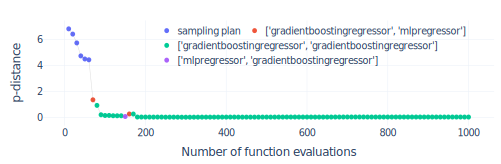
\includegraphics[width=\textwidth]{content/images/zdt6_models}
        \caption[ZDT6: Best models from the portfolio]{ZDT6: Best models from the portfolio}
        \label{fig:zdt6_models}
    \end{figure} 
    
    % The consistently low number of non-dominant solutions obtained by NSGA2 explains the slow convergence to the Pareto front. The figures above show the values that NSGA2 reached after 10000 function evaluations.
    % % The surrogate model can significantly accelerate the ascent to the global optimum. 
    % Let us take a look at TutorM and the validation results of the surrogate portfolio. As can be seen in Figure \ref{fig:zdt6_models}, there is an example of a sampling plan and three different compositional surrogate models. 

    
    The final solution consists of non-dominant configurations that give an idea of the Pareto front. In terms of overall Pareto front approximations (Figure \ref{fig:zdt6_front}), only TutorM solutions reach the baseline (NSGA2 10k) while other solutions are close and distributed (Hypermapper) or far away and clustered (NSGA2).

        % ===================== ZDT6: Front
        \begin{figure}[h]
            \centering   
            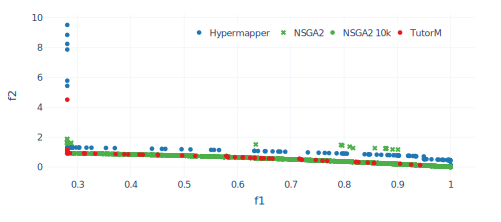
\includegraphics[width=\textwidth]{content/images/zdt6_front}
            \caption[The final assumption of the Pareto optimal solutions (1000 function evaluations) for ZDT6]{The final assumption of the Pareto optimal solutions (1000 function evaluations) for ZDT6}
            \label{fig:zdt6_front}
        \end{figure}

    % ----------------------------------------------------------- Case study's overview
    \subsection*{Case studies: WFG1, WFG4, DTLZ4}
    Below, we compare how the optimization process varied across several problems.
    The key feature of the method we developed is the dynamic sampling plan, which depends on the quality of available surrogates. 
    As mentioned before, in Figure \ref{fig:zdt6_models}, when a static number of random samples is estimated, it is possible to make optimal decisions much earlier.         
    
    This approach is used in TutorM for all optimization problems. By interpreting the end of the sampling plan and the availability of valid models, we can estimate the cross-grain complexity of the unknown problem. Figure \ref{fig:changing_models} shows a difference in the adaptation of initial samples to problems (DTLZ4, WFG1) and a corresponding improvement in hypervolume. 
    
        % === TutorM: surrogate portfolio in action
        \begin{figure}[!h]
            \centering
            \begin{subfigure}{\textwidth} 
                \includegraphics[width=\textwidth]{content/images/dtlz4_models}
                \caption{DTLZ4: sampling plan with 210 configuration}
                \label{fig:dtlz4_models_210}
            \end{subfigure}
            % \hfill
            
            \begin{subfigure}{\textwidth}
                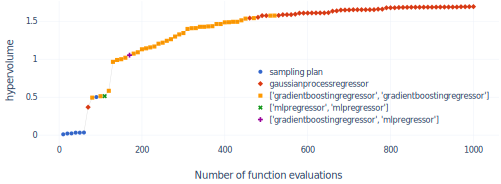
\includegraphics[width=\textwidth]{content/images/wfg1_models}
                \caption{WFG1: sampling plan with 60 configuration}
                \label{fig:wfg1_models_60}
            \end{subfigure} 
    
            \caption[Optimization process with dynamic sampling plan and surrogate portfolio.]{Optimization process with dynamic sampling plan and surrogate portfolio. Plots show in which steps a sampling plan was used or which model gives the best accuracy on the test set. The order of the models in the composite surrogates corresponds to the order of the optimization objectives that this model extrapolates.}
            \label{fig:changing_models}    
        \end{figure}
    
    
    In the case of WFG1, a valid model was quickly obtained and reduced the initial sampling. This may indicate a convenient and unimodal optimization landscape. On the contrary use-case of DTLZ4, the sampling plan lasted longer and alternated with valid models. This may reflect the complexity of the problem, such as the multimodality or bias of the landscape. It should also be noted that in each case we considered, the best surrogate model was different and might change during optimization. Thus, for the case of DTLZ4, a clear advantage was observed in the choice of composite surrogacy with \emph{Gradient Boosting Regressor}, whereas for WFG1, the multi-objective \emph{Gaussian Process Regressor} was the preferred choice.


    In the next comparison, we look at WFG1 and WFG4. Figure \ref{fig:wfg14} illustrates how the evaluation budget can be spent to find Pareto optimal solutions. Let us look at the WFG1. It can be seen that TutorM slowly increases the number of solutions during optimization (\ref{fig:wfg1_ndf}). Furthermore, the final result even exceeds the solutions given by the NSGA2 after 10k function evaluations (\ref{fig:wfg1_front}). Turning now to Hypermapper, the non-dominated plot is highly serrated, which indicates that the approach falls within the local optima. Additional information is revealed in the final Figure \ref{fig:wfg1_front}, which shows that most final Hypermapper solutions are strongly clustered, reflecting a waste of resources.

    For the WFG4 use-case, all approaches produce near-optimal solutions, but only TutorM provides such an extensive set of near-optimal solutions (non-dominated 400 solutions from 1000 function evaluations). This property of TutorM means that the optimization process can stop earlier and save on the evaluation budget.

    % === WFG1 and WFG4
    \begin{figure}[!h]
        \centering
        \begin{subfigure}{\textwidth}
            \begin{subfigure}{0.5\textwidth}
                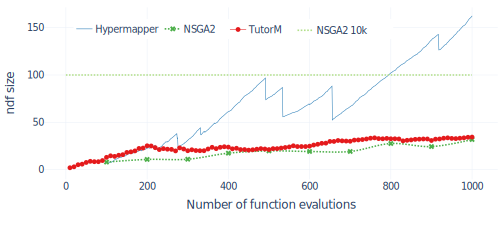
\includegraphics[width=\textwidth]{content/images/wfg1_ndf}
                \caption{Results of 5 repetitions for WFG1: Size of a non-dominated subset of evaluated examples}
                \label{fig:wfg1_ndf}
            \end{subfigure} 
            \begin{subfigure}{0.5\textwidth}
                \includegraphics[width=\textwidth]{content/images/wfg1_front}
                \caption{WFG1: Pareto front approximation}
                \label{fig:wfg1_front}
            \end{subfigure} 
        \end{subfigure} 
        \begin{subfigure}{\textwidth}
            \begin{subfigure}{0.5\textwidth}
                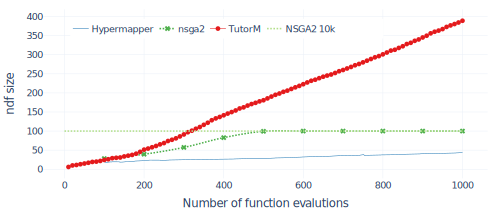
\includegraphics[width=\textwidth]{content/images/wfg4_ndf}
                \caption{Results of 5 repetitions for WFG4: Size of a non-dominated subset of evaluated examples}
                \label{fig:wfg4_ndf}
            \end{subfigure} 
            \begin{subfigure}{0.5\textwidth}
                \includegraphics[width=\textwidth]{content/images/wfg4_front}
                \caption{WFG4: Pareto front approximation}
                \label{fig:wfg4_front}
            \end{subfigure}
        \end{subfigure} 
        \caption[Comparison of WFG problems with the average number of non-dominant solutions and the final representation these to the Pareto Front.]{Comparison of WFG problems with the average number of non-dominant solutions and the final representation these to the Pareto Front}
        \label{fig:wfg14}    
    \end{figure}

% ---------------------------------------------------------- Results
    \subsection*{Results}

    For benchmark 1, we analyze 21 problems from three test sets. They have 2 or 3 parameters and 2 objectives. We repeat the experiments 5 times and average them. We consider the following metrics:
    \begin{itemize}
        \item \textbf{Hypervolume} This metric is calculated for each comparison because the hypervolume requires a single reference point for a group of competitors. Hypervolume metric is given as a percentage where $100\%$ corresponds to the maximum volume in the competition and $0\%$ corresponds to the hypervolume of a random set of solutions.
        \item \textbf{p-distance} The primary metric for evaluation that corresponds to average distance to real Pareto front. Unfortunately, it is not available for WFG problems.
        \item \textbf{Non-dominated font (ndf) size} The ratio of the number of final non-dominated decisions to the number of spent function evaluations.
        \item \textbf{Spacing} The inverse spacing metric is calculated, where 1 corresponds to the most cohesive decisions among competitors.
    \end{itemize}

    In Table \ref{tab:magic_five}, we present a subgroup of problems that have varying complexity. The full list of results is provided in the  \hyperref[sec:appendix-a]{appendix A}.

    % Please add the following required packages to your document preamble:
% \usepackage{booktabs}
% \usepackage{multirow}
% \usepackage[table,xcdraw]{xcolor}
% If you use beamer only pass "xcolor=table" option, i.e. \documentclass[xcolor=table]{beamer}
\begin{table}[]
    \centering
    \begin{tabular}{@{}lllllll@{}}
    \toprule
                                                                                              & Metric      & ZDT4                                     & ZDT6                                     & DTLZ4                                     & WFG1                                     & WFG4                                     \\ \midrule
                                                                                              & \textbf{Hypervolume} $\uparrow$  & \cellcolor[HTML]{EFEFEF}\textbf{99,8\%} & \cellcolor[HTML]{EFEFEF}\textbf{99,43\%} & \cellcolor[HTML]{EFEFEF}\textbf{99,83\%} & \cellcolor[HTML]{EFEFEF}\textbf{95,75\%} & \cellcolor[HTML]{EFEFEF}\textbf{99,28\%} \\
                                                                                              & \textbf{p-distance} $\downarrow$  & \cellcolor[HTML]{EFEFEF}\textbf{0,01}    & \cellcolor[HTML]{EFEFEF}\textbf{0,09}    & \cellcolor[HTML]{EFEFEF}\textbf{0,001}    & -                                        & -                                        \\
                                                                                              & \textbf{ndf-size} $\uparrow$     & \cellcolor[HTML]{EFEFEF}\textbf{50\%}                          & 4,26\%                                   & 0,2\%                                     & 3,44\%                                   & \cellcolor[HTML]{EFEFEF}\textbf{38,9\%} \\
    \multirow{-4}{*}{\textbf{TutorM}}                                                         & \textbf{spacing} $\uparrow$      & \cellcolor[HTML]{EFEFEF}\textbf{0,78}    & \cellcolor[HTML]{EFEFEF}\textbf{0,17}    & \cellcolor[HTML]{EFEFEF}\textbf{0,66}    & \cellcolor[HTML]{EFEFEF}\textbf{0,51}    & \cellcolor[HTML]{EFEFEF}\textbf{1}       \\ \midrule
                                                                                              & \textbf{Hypervolume} $\uparrow$  & 83,43\%                                  & 83,84\%                                  & 87,807\%                                  & 30,52\%                                  & 83,95\%                                  \\ 
                                                                                              & \textbf{p-distance} $\downarrow$  & 0,04                                     & 1,29                                     & 0,002                                     & -                                        & -                                        \\
                                                                                              & \textbf{ndf-size} $\uparrow$     & 8,77\%                                   & 1,01\%                                   & \cellcolor[HTML]{EFEFEF}\textbf{9,6\%}    & 3,18\%                                   & 10\%                                     \\
    \multirow{-4}{*}{\textbf{NSGA2}}                                                          & \textbf{spacing} $\uparrow$      & 0,19                                     & 0,04                                     & 0,323                                     & 0,28                                     & 0,58                                     \\ \midrule
                                                                                              & \textbf{Hypervolume} $\uparrow$  & 97,32\%                                  & 82,86\%                                  & 64,57\%                                   & 44,12\%                                  & 84,39\%                                  \\ 
                                                                                              & \textbf{p-distance} $\downarrow$  & 0,90                                     & 1,12                                     & 0,059                                     & -                                        & -                                        \\
                                                                                              & \textbf{ndf-size} $\uparrow$     & 5,42\%                                   & \cellcolor[HTML]{EFEFEF}\textbf{6,25\%}  & 1,177\%                                   & \cellcolor[HTML]{EFEFEF}\textbf{10,24\%} & 3,26\%                                   \\
    \multirow{-4}{*}{\textbf{Hypermaper 2.0}}                                                     & \textbf{spacing} $\uparrow$      & 0,11                                     & 0,08                                     & 0,029                                     & 0,31                                     & 0,06                                     \\ \midrule
                                                                                              & \textbf{Hypervolume} $\uparrow$  & 100\%                                    & 100\%                                    & 100\%                                     & 100\%                                    & 100\%                                    \\  
                                                                                              & \textbf{p-distance} $\downarrow$  & 2,04e-05                                 & 0,0003                                   & 8,81e-06                                  & -                                        & -                                        \\
                                                                                              & \textbf{ndf-size} $\uparrow$     & 0,72\%                                   & 0,72\%                                   & 0,36\%                                    & 0,72\%                                   & 0,72\%                                   \\ 
    \multirow{-4}{*}{\textbf{\begin{tabular}[c]{@{}l@{}}NSGA2 50k\\ (Baseline)\end{tabular}}} & \textbf{spacing} $\uparrow$      & 1                                        & 1                                        & 1                                         & 1                                        & 0,6                                     \\ \bottomrule
    \end{tabular}
    \caption{Comparison of results after 1000 feature evaluations}
    \label{tab:magic_five}
    \end{table}

        % \begin{table}[]
    %     \centering
    %     \caption{Comparison of final results after 1000 feature evaluations}
    %     \resizebox{\textwidth}{!}{%
    %     \begin{tabular}{@{}ccccccc@{}}
    %     \toprule
    %                                          & \textbf{Metric}        & \textbf{ZDT4} & \textbf{ZDT6} & \textbf{DTLZ4} & \textbf{WFG1} & \textbf{WFG4} \\ \midrule
    %     \multirow{4}{*}{\textbf{TutorM}}     & \textbf{hypervolume}   & 99,45\%       & 99,01\%       & 99,27\%        & 115,60\%      & 95,95\%       \\
    %                                          & \textbf{p-distance}    & 1,336         & 0,522         & 0,022          & -             & -             \\
    %                                          & \textbf{ndf-size}      & 183,022       & 31,528        & 119,308        & 24,158        & 183,244       \\
    %                                          & \textbf{space-metrics} & 0,103         & 0,142         & 0,186          & 0,129         & 0,032         \\ \midrule
    %     \multirow{4}{*}{\textbf{NSGA2}}      & \textbf{hypervolume}   & 97,57\%       & 87,46\%       & 95,87\%        & 45,01\%       & 91,87\%       \\
    %                                          & \textbf{p-distance}    & 1,391         & 1,872         & 0,022          & -             & -             \\
    %                                          & \textbf{ndf-size}      & 44,000        & 11,455        & 39,900         & 20,164        & 82,436        \\
    %                                          & \textbf{space-metrics} & 0,176         & 0,355         & 0,268          & 0,228         & 0,038         \\ \midrule
    %     \multirow{4}{*}{\textbf{Hypermaper}} & \textbf{hypervolume}   & 96,82\%       & 66,95\%       & 81,29\%        & 40,66\%       & 74,09\%       \\
    %                                          & \textbf{p-distance}    & 2,024         & 1,850         & 0,076          & -             & -             \\
    %                                          & \textbf{ndf-size}      & 28,908        & 52,746        & 10,743         & 81,512        & 30,158        \\
    %                                          & \textbf{space-metrics} & 0,1386        & 0,11621       & 0,5282         & 0,0870        & 0,1032        \\ \midrule
    %     \multirow{4}{*}{\textbf{\begin{tabular}[c]{@{}c@{}}NSGA2\\ 10k eval\end{tabular}}} & \textbf{hypervolume}      & 100,00\% & 100,00\% & 100,00\% & 100,00\% & 100,00\% \\
    %                                          & \textbf{p-distance}    & 0,152         & 0,256         & 0,002          & -             & -             \\
    %                                          & \textbf{ndf-size}      & 93,901        & 79,776        & 93,990         & 85,196        & 98,087        \\
    %                                          & \textbf{space-metrics} & 0,033         & 0,074         & 0,039          & 0,051         & 0,016         \\ \bottomrule
    %     \end{tabular}%
    %     }
    % \label{tab:magic_five} 
    % \end{table}


    To summarize, it follows from our results that our strategy generally gives optimal or better results than the baseline on the majority of investigated problems.
    

    We assume that our positive results were due to the new features we implemented, such as a surrogate model portfolio and adaptive sampling plan. These features have yielded significant results on almost all problems. However, we did not apply inner parameter tuning: in all experiments, TutorM was used with default parameters.

% --------------------------------------------------------------------------------------------
% ---------------------       Benchmark 2: Dynamic sampling plan and parameter selection
% --------------------------------------------------------------------------------------------
\section{Benchmark 2: Inner parameters } \label{sec:bench2}
    For the second benchmark, we investigated whether it is possible to further improve the performance of TutorM by tuning its parameters. We examine the effect of internal parameters on the performance and quality of optimization. As was mentioned in the previous section, it was applied with a default setting.

    \subsection{TutorM parameters}
    Besides the standard model-based parameters, it is necessary to investigate the impact of additional TutorM parameters such as validation thresholds, test-set and prediction size. This research is needed to select the configuration that can improve results of the existing system. Unfortunately, there is insufficient information available about how to configure model-based parameter optimization \cite{TobiasCV, HybridSurrRCG}. Filling this gap in knowledge will be useful not only for the availability of TutorM but also for general tuning of model-based optimization.  
    Due to limited time, we consider only the ZDT4 and ZDT6 problems using the surrogate portfolio from the first benchmark, but without the \emph{Gaussian regression model}. This model takes a long time to train and the full factorial design did not fit within our time frame.
    % Secondly, hyperparameter tuning for a spe- cific model class, selecting from a finite amount of different models and possibly choosing relevant features are important steps in practical optimization. It

    The following parameters are exposed in the developed TutorM class:
    \begin{itemize}
        \item \textbf{Initial dataset} [\underline{0}, 100, 500, 750]. It is the initial number of points obtained from sampling plan. At the same time, the total budget for measurements remains unchanged and equals 1000. The default value is 0.
        \item \textbf{Surrogate validation.} Criteria and parameters for evaluating the usefulness of the surrogate model.
            \begin{itemize}
                \item \textbf{Train/test split} [\underline{75/25}, 90/10] is a splitting proportion in which the samples available for training and testing are divided. Train and test sets are crucial to ensure that the surrogate model is able to generalize well to new data. The default value is 75/25.
                \item \textbf{Cross-validation threshold}[0.2, \underline{0.65}, 0.9] is a minimum accuracy threshold for any round in cross-validation(CV). CV is used to select valid surrogate models and avoid overfitting. The default values is 0.65.
                \item \textbf{Test threshold} [0, \underline{0.6}, 0.9] is a minimum accuracy threshold for the test set. The accuracy obtained from the test set and is used to verify the validity of models based on how they extrapolate unknown data. The default value is 0.6.
            \end{itemize}
    \item \textbf{Optimization search algorithm} [NSGA2, \underline{MOEA-Ctrl}] optimization algorithm for multi-objective solutions. The default value is MOEA-Ctrl.
    \item \textbf{Solution combinations} [Non-dominated front score (ndf score), \underline{Stacking}] approach for choosing a set of solutions from a valid surrogate model. Since several models can be valid and each one provides its own set of decisions, we have a range of options. \emph{Non-dominated front score (ndf score)} prefers the surrogate model with the highest precision for non-dominant solutions, whereas the \emph{stack} integrates all available surrogate solutions into one set of solutions. The default value is Stacking.
    \item \textbf{Prediction count} [\underline{10}, 100] number of random solutions for the real evaluation that are selected from the set of solutions. The default value is 10.
    \end{itemize}

    As a result of the full factorial design, 576 possible combinations were obtained. Each combination was repeated five times and averaged. Conclusions were made based on the 40 best and worst combinations.

    % ---------------------------------------------- ZDT6
    First, we will consider the ZDT6 problem. Inspection of Figure \ref{fig:conf_zdt6} indicates that the \emph{solution combination} made the most significant impact on the result. 

            % ===  ------------------------------------- ZDT6
            \begin{figure}[h!]
                \centering
                \begin{subfigure}{\textwidth}
                    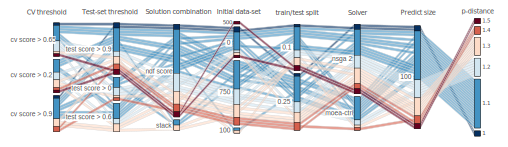
\includegraphics[width=\textwidth]{content/images/conf_zdt6_worst}
                    \caption{40 worst configurations}
                    \label{fig:conf_zdt6_worst}
                \end{subfigure} 
                % \hfill
                
                \begin{subfigure}{\textwidth}
                    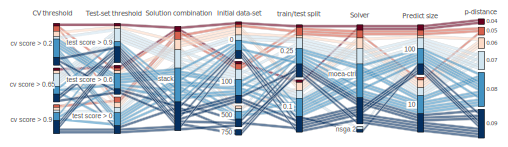
\includegraphics[width=\textwidth]{content/images/conf_zdt6_best}
                    \caption{40 best configurations}
                    \label{fig:conf_zdt6_best}
                \end{subfigure}   
                \caption[ZDT6: Average result of the best and worst configurations.]{ZDT6: Average result of the best and worst configurations.}
                \label{fig:conf_zdt6}    
            \end{figure}
    There is a definite advantage in combining solutions into a stack. The second most important parameter is the \emph{Optimization search algorithm}(Solver). The best configurations prefer to pick a combination of Genetic Algorithms (MOEA-Ctrl) for optimization.
    
    Let us look at the \emph{solution combination} and the \emph{Optimization search algorithm} options in more detail (Figure \ref{fig:conf_zdt6_sign}). 
    
            % === ZDT 6
            \begin{figure}[h!]
                \centering
                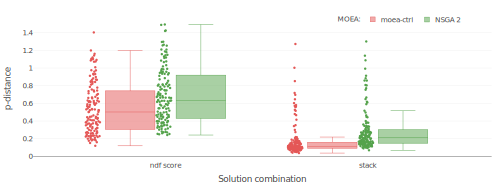
\includegraphics[width=0.8\textwidth]{content/images/conf_zdt6_solver}
                \caption[Correlation between the most influenceable parameters for the ZDT6]{Correlation between the most influenceable parameters for the ZDT6: solution combination strategy and optimization algorithm}
                \label{fig:conf_zdt6_sign}    
            \end{figure}
    
    The impact of changing the algorithm is highly dependent on the solution combination strategy. Improvement in results for MOEA-Ctrl is more significant when the results are combined into a stack. This advantage can be explained by the fact that the stack reduces the bias of surrogate models while the combination of genetic algorithms decreases prediction variance.



    % ---------------------------------------------- ZDT4
    Now we will look at the ZDT4 problem (Figure \ref{fig:conf_zdt4}). 
    
            % === -------------------------------------- ZDT 4
            \begin{figure}[h!]
                \centering
                \begin{subfigure}{\textwidth}
                    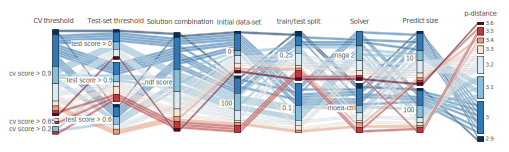
\includegraphics[width=\textwidth]{content/images/conf_zdt4_worst}
                    \caption{40 worst configurations}
                    \label{fig:conf_zdt4_worst}
                \end{subfigure} 
                % \hfill       
                \begin{subfigure}{\textwidth}
                    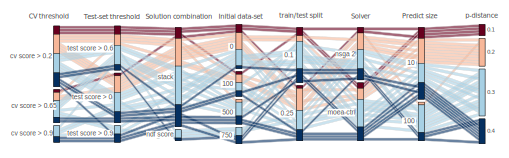
\includegraphics[width=\textwidth]{content/images/conf_zdt4_best}
                    \caption{40 best configurations}
                    \label{fig:conf_zdt4_best}
                \end{subfigure} 
        
                \caption[ZDT4: Average results of best and worst configurations.]{ZDT4: Average results of best and worst configurations.}
                \label{fig:conf_zdt4}    
            \end{figure}
    
    The results are similar to those obtained with the ZDT6 problem: the solutions stack take part almost in all of the best configurations. However, for this problem, there is no clear dominance of a single algorithm. Yet, the validation thresholds have an impact on results (Figure \ref{fig:conf_zdt4_sign}). 

        % === ZDT4
        \begin{figure}[h!] 
            \centering
            % \begin{subfigure}{0.3\textwidth}
            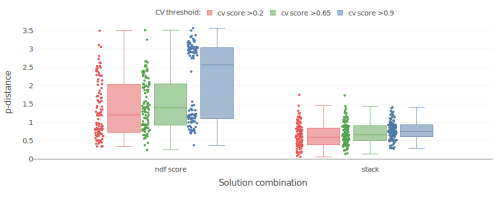
\includegraphics[width=0.90\textwidth]{content/images/conf_zdt4_cv_score}
                % \caption{An impact of the cross-validation threshold}
                % \label{fig:zdt4_pred_solver}
            % \end{subfigure} 
            % \begin{subfigure}{0.3\textwidth}
            %     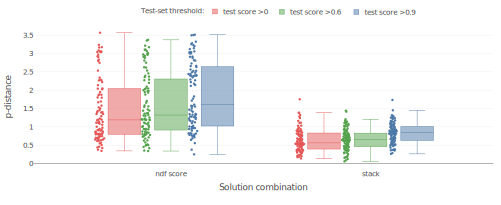
\includegraphics[width=\textwidth]{content/images/conf_zdt4_test_score}
            %     \caption{An impact of the test-set-validation threshold}
            %     \label{fig:zdt4_comb_valid}
            % \end{subfigure}
            \caption[An impact of the cross-validation threshold for the ZDT4]{An impact of the cross-validation threshold for the ZDT4} 
            \label{fig:conf_zdt4_sign}    
        \end{figure}


    A significant difference is seen for the cross-validation threshold in the case of \textit{ndf score} \emph{solution combination} set (Figure \ref{fig:conf_zdt4_worst}). It should be noted that the stack makes the validation threshold impact less significant, as evident from Figure \ref{fig:conf_zdt4_sign}. This influence is related to this technique's ability to reduce the bias of solutions. 
    
    Another interesting conclusion can be made from the \emph{initial sample size}. The worst and the best configurations are most affected by tha absence of a sampling plan. The reason for this is that the small number of samples may lead to a surrogate model fallacy in extrapolation the search space while, at the same time, the small number of samples provide more opportunities for optimization search.

    % ====================================================== Start set for Hypermapper 2.0
    \subsection{Sampling plan size}
    The purpose of this experiment is to review the dependencies between the optimization results and the sampling plan size. The Hypermapper was selected as a foundation for analysis because it has a static implementation of the optimization algorithm with the surrogate model.

    The results are shown in the following Figure \ref{fig:hmapper_start_set}. 
    
    \begin{figure}[!h]
        \centering
        \begin{subfigure}{\textwidth}
            \begin{subfigure}{0.45\textwidth}
                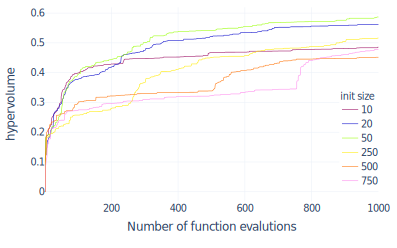
\includegraphics[width=\textwidth]{content/images/hypermapper_wfg1_start_set}
                \caption{WFG1}
                \label{fig:hmapper_wfg1_start_set}
            \end{subfigure}
            \begin{subfigure}{0.45\textwidth}
                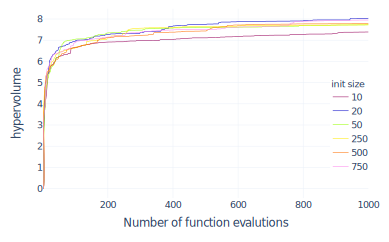
\includegraphics[width=\textwidth]{content/images/hypermapper_wfg4_start_set}
                \caption{WFG4}
                \label{fig:hmapper_wfg4_start_set}
            \end{subfigure}
        \end{subfigure} 
        \hfill

        
        \begin{subfigure}{\textwidth}
            \begin{subfigure}{0.45\textwidth}
                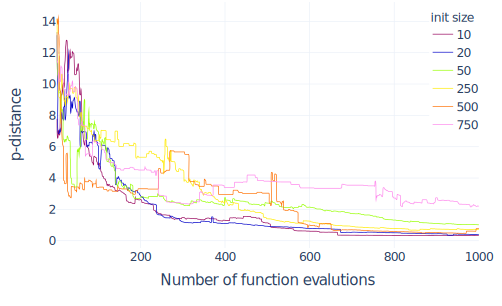
\includegraphics[width=\textwidth]{content/images/hypermapper_zdt4_start_set}
                \caption{ZDT4}
                \label{fig:hmapper_zdt4_start_set}
            \end{subfigure}
            \begin{subfigure}{0.45\textwidth}
                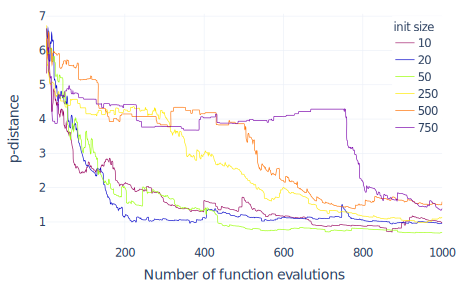
\includegraphics[width=\textwidth]{content/images/hypermapper_zdt6_start_set}
                \caption{ZDT6}
                \label{fig:hmapper_zdt6_start_set}
            \end{subfigure}
        \end{subfigure} 

        \caption[Influence of the initial sample plan on optimization process with Hypermapper 2.0]{Influence of the initial sample plan on optimization process with Hypermapper 2.0}
        \label{fig:hmapper_start_set}    
    \end{figure}
    
    
    For WFG problems, the criterion is hypervolume and for ZDT problems it is p-distance. Of all the results, the initial sampling plan has the smallest effect on the WFG4. Since this problem is unimodal, the model requires fewer samples for extrapolation. Other problems have a more complicated multimodal landscape that is shown by unstable results. 


    % -------------------------------------------------   Results
    \subsection*{Results}
    We investigated the parameters of TutorM and determined which ones produce the best results. Also was noticed that \emph{Solution combinations} and \emph{Optimization search algorithm} had the most significant impact on solution quality. The \emph{stack} of solutions with MOEA-Ctrl is the best combination of parameters to use as a default for TutorM. 
    The other parameters tested have a much smaller effect.


% --------------------------------------------------------------------------------------------
% ---------------------       Benchmark 3: Many-objective optimization, scaling
% --------------------------------------------------------------------------------------------
\section{Benchmark 3: Scalability of surrogate models}
    Not only the type of the problem landscape but also its dimensions are essential factors for picking a surrogate model. The advantage of a surrogate model can be lost if the number of parameters or criteria is changed. The goal of this experiment is to find out the scalability of surrogate models.  

    The following surrogates were selected for evaluation:
    \begin{itemize}
        \item \emph{Gaussian Process Regressor} with kernel design from GPML\cite{RasmussenN10}. Gaussian process models are well-known and are commonly used in Bayesian optimization for a wide variety of problems \cite{EmmerichGN06, MlakarPTF15}. 
        \item \emph{MLPRegressor} is a neural network implementation from the \textit{sklearn} framework. Neural networks can automatically discover useful representations in high-dimensional data by learning multiple layers \cite{WilsonHSX16}. Because this model simultaneously extrapolates all objectives, we chose an architecture that consists of 5 layers and 100 neurons per layer.
        \item The surrogate portfolio includes Gradient Boosting Regressor, MLPRegressor, and \emph{SVR (RBF kernel)}, as mentioned in Section \ref{sec:bench2}.
    \end{itemize}

    The DTLZ2 problem was selected to evaluate the scalability of the surrogate models. It is an unimodal problem with multiple global optima and concave geometry of the Pareto front. 
    During experimentation with DTLZ2, the number of optimization criteria changed with a constant number of parameters. Figure \ref{fig:scale_dtlz2} shows the three selected surrogate strategies with the average distance to the Pareto front (first row) and time spent per optimization iteration (bottom row). For all cases, the experiment was repeated five times. 

        % ------------------ Scale DTLZ 
        \begin{figure}[h]
            \centering
            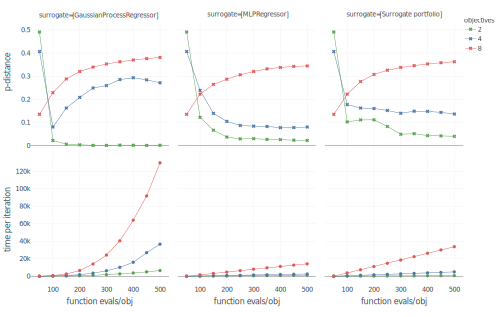
\includegraphics[width=\textwidth]{content/images/scale_dtlz2}
            \caption[Scaling example for the three variants of the surrogate on the DTLZ2.]{Scaling example for the three variants of the surrogate on the DTLZ2 with the 9-dimensional parameter space.}
            \label{fig:scale_dtlz2}    
        \end{figure}

    As illustrated by Figure \ref{fig:scale_dtlz2}, \emph{Gaussian Process Regressor} model provides significantly better results relative to other approaches, but only for the bi-objective problem. Increasing the number of objectives to four leads to only the \emph{MLPRegressor} and surrogate portfolio converging on an optimal solution. Further increasing the number of objectives makes the search space too complicated, and all approaches fail to find solutions.
    
    \subsection*{Results}
    The ability of models to estimate the search space depends on their hyperparameters. As an example: \emph{Gaussian Process Regressor} are highly dependent on the kernel while \emph{MLPRegressor} depends on a number of layers.
    In turn, for the surrogate portfolio, the parameters determine how to \emph{build and select} surrogate models. In the portfolio, a single model with varying parameters is evaluated as a set of separate entities. Thus, the scalability required to solve multi-dimensional problems can be generated by surrogate portfolios.


% --------------------------------------------------------------------------------------------
% ------------------------------------------------     Discussion 
% --------------------------------------------------------------------------------------------
\section{Discussion of results}

The purpose of this thesis is to investigate the use of a cross-grained compositional model for solving multi-objective problems. In this evaluation section, we provided an extensive comparative analysis of the performance of our and other techniques on a wide range of problems. The analysis also included an exhaustive study of the possible parameters and the impact of the sampling plan on results. The possibility of scaling surrogate models by increasing the number of objectives was also tested. We draw the following conclusions from our evaluation experiments:
\begin{enumerate}
    \item TutorM is far ahead of its counterparts (Hypermapper 2.0 and NSGA2) and achieves optimal results while sparing function evaluations. 
    %Are my modifications accurate? I removed the second sentence because it seemed redundant, and less assertive than the first sentence.
    \item Parameter analysis for TutorM shows that results are significantly improved by combining solutions with multiple surrogates (solution stack).
    \item When the possibility of scaling up the surrogate portfolio was tested, we determine that dynamically selecting an appropriate surrogate model for the specific dimensionality of the problem is essential.
\end{enumerate}